\documentclass[main.tex]{subfiles}
% CONCEPTS
\begin{document}
  
  The derivative analysis builds mainly on a matrix, beginning with the actual data values (derivative 0), followed by the derivatives along the "depth" of the matrix. This is demonstrated in \cref{tbl:mtrx:simple} with a parabola. The depth that the matrix reaches before becoming zero in a particular column defines that data point's derivative depth or \textit{derivDepth}.

  \subfile{tables/simpleMatrix}
  
  \section{Derivative Characteristics}
    
    Due to its simplicity, most classification is best performed while making use of the polynomial classification.
    
    \begin{figure}[h]
      \begin{subfigure}{0.48\linewidth}
        \centering
        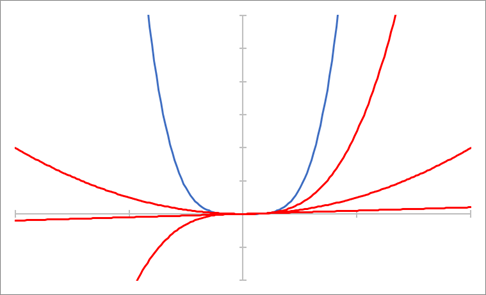
\includegraphics[width=0.9\linewidth]{figures/derivPoly}
        \caption{Polynomials}
        \label{fig:deriv:poly}
      \end{subfigure}
      \begin{subfigure}{0.48\linewidth}
        \centering
        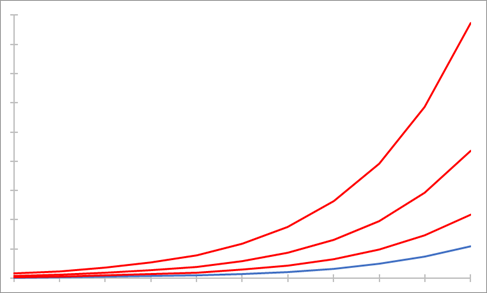
\includegraphics[width=0.9\linewidth]{figures/derivExp}
        \caption{Exponential}
        \label{fig:deriv:exp}
      \end{subfigure}
      \caption{Derivative patterns of (\subref{fig:deriv:poly}) polynomial and \subref{fig:deriv:exp}) exponential functions. (\subref{fig:deriv:poly}) shows a fourth order polynomial in blue ($x^4$) and its derivatives in red, a third ($x^3$), second ($x^2$) and first ($x$) order polynomial, which a "zeroth" order polynomial ($x^0$ or simply $1$) follows, but is too small do display. No further derivatives would follow. (\subref{fig:deriv:exp}) shows an exponential of the form $e^{a x}$ in blue, with $a>1$ and hence its derivatives growing larger with the level of derivative, by $a$, $a^2$ and $a^3$ respectively. (\subref{fig:deriv:exp}) will never reach a zero derivative.}
      \label{fig:deriv}
    \end{figure}
    
    \subsection{Polynomials}
    
      By far the simplest functions to classify are \textbf{polynomials}. Any polynomial of degree $N$ will have exactly $N$ non-zero derivatives (also see \cref{fig:deriv:poly}), and so it is only necessary to count the number of times that the derivative is not zero i.e. the \textit{derivDepth}. If it never becomes zero then the data is not polynomial, or we have not taken enough derivatives. \Cref{tbl:mtrx:simple} shows an example of a second order polynomial being classified.
      
    \subsection{Points of Interest}
      
      Within polynomial data segments POI can be detected by a characteristic \textit{POI-tail}, as can be seen in \cref{tbl:mtrx:poi}. As in the POI the derivative changes in a way that breaks the underlying pattern, characterised by its \textit{derivDepth}, which in turn propagates through the preceding points down the depth of the matrix. Typically this will form a triangle pattern, though at times it is only a diagonal line. This line, however, will always form whenever the definition of a \textit{Point of Interest} from \cref{sec:POI} is satisfied.
      
      \subfile{tables/poiMatrix}    
      
      Provided that the data segment is polynomial the POI-tail can simply be identified by checking for non-zero entries in the matrix at a depth beyond the \textit{derivDepth} already assigned to the data point. 
    
    \subsection{Nested Functions}
      \label{sec:con:nest}
      
      As stated in \cref{sec:back:combFunc}, there are limitations to the amount of analysis that can be performed on combined functions. However, the most common functions can be easily covered, by applying their inverse after classifying a segment as not-polynomial. First the Natural Logarithm is applied to the data segment in question, which is then analysed again. If it is classified as a polynomial at this stage the original data segment can be marked as exponential. While further analysis is not yet implemented, similar processes will allow classification of rational and root functions, as well as logarithmic functions.
      \\\\
      Note, however, in \cref{fig:deriv:exp}, how towards the left side the exponentials approximate to zero. All exponentials have such an asymptote, where they approximate a constant of zero to infinite precision. This is also demonstrated in \cref{tbl:mtrx:exp}. There is no mathematical means to tell this segment apart from a true constant, without the additional information from other data segments or infinite precision that no sensor can provide. At this time this classification is considered accurate, but it can be adjusted for in the next analysis step, when information from more than one data point at a time is used to continue analysis. Similar segments exist in logarithmic and rational functions.
      
      \subfile{tables/expMatrix}
      
  \section{Precision}
    
    In the context of this method, precision largely refers to the point at which differences between two data points are ignored. \Cref{tbl:mtrx:exp} makes use of a precision of $0.1$, for example, and as a result any data points or derivative values that are compared will produce zero whenever their difference is smaller than $0.1$. On the one hand higher precision would allow the method to more accurately classify functions. However, this accuracy is limited by the data quality. If the noise is too great then the method begins to classify order in the chaos, as is common when overstraining ML algorithms \cite{}. 
    \\\\
    Even in the final implementation precision is simply the amount of difference below which two values can be considered equal and hence their slope becomes zero. So long as noise does not exceed this value there should be no issue in ignoring it, while noise above this value would be classified as outlier \textit{POI}. As floating point errors are always negligible in comparison to noise in data, this also protects the software from running into floating point related issues.
%    \\\\
%    Naturally, precision poses a balancing problem between noise robustness and analytic power.
%    
%    Example table with too little precision
  
    \begin{figure}[h]
      \centering
      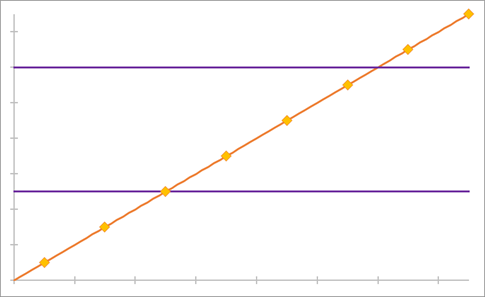
\includegraphics[width=0.6\linewidth]{figures/lowPrec}
      \caption{A hypothetical linear function that generates a data set (both orange), compared to a low precision setting (upper and lower bound in purple). When taking the derivative between points, any two points between the upper and lower bound are considered equal and will produce a zero derivative. Here this leads to a classification to a constant, as no difference between ppoints is detected.}
      % demonstrate noise
      \label{fig:lowPrec}
    \end{figure}
  
  
\end{document}